% !TEX root = ./xstream.tex

\section{Baselines}
\subsection{Datasets}
Datasets shown in Table~\ref{table:datasets}.

\begin{table}[]
\centering
\label{table:datasets}
\begin{tabular}{ccc}
\textbf{Dataset Name}         & \textbf{\#Samples} & \textbf{\#Features} \\	\hline \hline
breast-cancer-wisconsin (Mid) & 568                & 30                  \\
ionosphere (Mid)              & 350                & 33                  \\
magic-telescope (Low)         & 19020              & 10                  \\
pima-indians (Low)            & 768                & 8		\\
gisette (High) & 7000 & 4970	\\
isolet (High) & 7797 & 616		\\
letter-recognition (High) & 7797 & 616	\\
madelon (High) & 2600 & 500	\\
\end{tabular}
\caption{List of benchmark datasets used.}
\end{table}

\subsection{Adding Noise To Datasets}
We used $2$ different methods to generate benchmark datasets. The first method was applicable only to the low-dimensional and mid-dimensional datasets, and the second method was for high-dimensional datasets. We explain both of these methods below:
\textbf{Method 1}: We add noisy columns to the original dataset. The number of noisy columns is in the percentage of original number of columns that are added, and the noise level governs the mean and standard deviation of the gaussian distribution. We play around with percentage of noisy columns to be added, choosing values such as  100, 1000, 2000, and 5000. For noise-levels, we played with 0.01, 0.1, 0.2, 0.25. The mean and standard deviation of the Gaussian distribution was just noise-level multiplied with the original mean, or the original standard deviation of the entire dataset.

\textbf{Method 2}: We first discard all the original anomalous points. Now for the remaining nominal points, we first choose 10\% of the features and mark them as important features. We further proceed with choosing 5\% of the dataset as important samples. Now, in this sub-block, which contains only important samples and important features, we add Gaussian noise to the original data. Again, Gaussian noise is used, parameterized by the mean, and the standard deviation of the entire nominal dataset. Further this noise is scaled according to the user-specified signal to noise ratio, and added to the original sub-block of our dataset and features.

\subsection{Baseline Algorithms}
\begin{itemize}
\item{\textbf{iForest}: We use it with recommended sample size of $256$ or the entire dataset, whichever is minimum. The hlim is set to $15$ to be comparable to HS-Trees, and number of components is set to $100$.}
\item{\textbf{HS-Trees}:  Use it with recommended setting of $15$ max depth trees, and number of components is $100$.}
\item{\textbf{LODA}: We set the sparsity factor to $\frac{1}{\sqrt(d)}$. We allow LODA to select best width for histograms, but fix the number of histograms to $100$ to be comparable to rest of the algorithms.}
\item{\textbf{RS-Hash}: For RS-Hash, we use $1000$ sampling points, as recommended and $100$ components.}
\end{itemize}

\subsection{Baseline Results}
\begin{footnotesize}
\begin{table}[p!]
    %\centering
		\begin{tabular}{lcccccc}
				\toprule
				\textbf{Dataset} & \textbf{IF} &  \textbf{LODA} & \textbf{RSH} &  \textbf{HST}  & \textbf{XS}\\
				\midrule
				\multicolumn{6}{c}{\textit{High-dimensional Datasets}}\\
%gisette& $0.423 \pm 0.011$ &  $0.436 \pm 0.008$ &  $0.417 \pm 0.005$ &  $0.432 \pm 0.017$    \\
gisette (30,0.3,1.2)  & $0.683 \pm 0.045$ &  $0.531 \pm 0.018$ &  $0.460 \pm 0.005$ &  $0.628 \pm 0.021$  & $0.528 \pm  0.009$ \\
gisette (30,0.3,10)   & $0.541 \pm 0.027$ &  $0.321 \pm 0.004$ &  $0.354 \pm 0.002$ &  $0.471 \pm 0.024$  & $0.320 \pm  0.003$   \\
gisette (30,0.3,20)   & $0.450 \pm 0.022$ &  $0.290 \pm 0.003$ &  $0.308 \pm 0.003$ &  $0.347 \pm 0.017$  & $0.292 \pm  0.003$  \\
gisette (30,0.3,30)   & $0.432 \pm 0.016$ &  $0.301 \pm 0.005$ &  $0.310 \pm 0.002$ &  $0.316 \pm 0.006$  & $0.293 \pm  0.002$  \\
\midrule
%isolet& $0.442 \pm 0.019$ &  $0.429 \pm 0.02$ &  $0.444 \pm 0.001$ &  $0.444 \pm 0.013$    \\
isolet (30.0,0.3,1.2) & $0.537 \pm 0.03$  &  $0.580 \pm 0.030$ &  $0.441 \pm 0.01$  &  $0.559 \pm 0.028$  & $0.640 \pm  0.020$   \\
isolet (30.0,0.3,10)  & $0.372 \pm 0.011$ &  $0.350 \pm 0.007$ &  $0.334 \pm 0.004$ &  $0.391 \pm 0.015$  & $0.348 \pm  0.007$  \\
isolet (30.0,0.3,20)  & $0.330 \pm 0.009$ &  $0.313 \pm 0.006$ &  $0.311 \pm 0.001$ &  $0.322 \pm 0.007$  & $0.318 \pm  0.002$   \\
isolet (30.0,0.3,30)  & $0.300 \pm 0.002$ &  $0.292 \pm 0.004$ &  $0.296 \pm 0.001$ &  $0.293 \pm 0.002$  & $0.290 \pm  0.002$  \\
\midrule
%letter-recognition& $0.475 \pm 0.012$ &  $0.46 \pm 0.011$ &  $0.453 \pm 0.003$ &  $0.471 \pm 0.009$    \\
letter (30.0,0.3,1.2) & $0.490 \pm 0.026$ &  $0.534 \pm 0.03$  &  $0.440 \pm 0.010$ &  $0.519 \pm 0.053$ & $0.597 \pm  0.020$   \\
letter (30.0,0.3,10)  & $0.374 \pm 0.015$ &  $0.337 \pm 0.003$ &  $0.339 \pm 0.008$ &  $0.375 \pm 0.007$ & $0.336 \pm  0.005$   \\
letter (30.0,0.3,20)  & $0.309 \pm 0.008$ &  $0.289 \pm 0.002$ &  $0.291 \pm 0.002$ &  $0.310 \pm 0.007$ & $0.300 \pm  0.002$   \\
letter (30.0,0.3,30)  & $0.319 \pm 0.01$  &  $0.305 \pm 0.003$ &  $0.308 \pm 0.001$ &  $0.307 \pm 0.004$ & $0.310 \pm  0.002$   \\
\midrule
%madelon& $0.501 \pm 0.008$ &  $0.515 \pm 0.014$ &  $0.507 \pm 0.003$ &  $0.511 \pm 0.01$    \\
madelon (5.0,0.05,1.2)& $0.896 \pm 0.051$ &  $1.000 \pm 0.0$   &  $0.920 \pm 0.007$ &  $0.969 \pm 0.039$ & $1.000 \pm  0.000$   \\
madelon (5.0,0.05,10) & $0.643 \pm 0.13$  &  $0.988 \pm 0.012$ &  $0.784 \pm 0.068$ &  $0.899 \pm 0.094$ & $0.957 \pm  0.023$   \\
madelon (5.0,0.05,20) & $0.240 \pm 0.093$ &  $0.112 \pm 0.027$ &  $0.160 \pm 0.039$ &  $0.377 \pm 0.143$ & $0.125 \pm  0.013$  \\
madelon (5.0,0.05,30) & $0.070 \pm 0.013$ &  $0.054 \pm 0.007$ &  $0.083 \pm 0.004$ &  $0.099 \pm 0.059$ & $0.044 \pm  0.003$   \\
\midrule
\multicolumn{6}{c}{\textit{Low/medium-dimensional Datasets}}\\
breast-cancer (100,0.1)   & $0.661 \pm 0.036$ &  $0.839 \pm 0.024$ &  $0.727 \pm 0.010$ &  $0.702 \pm 0.026$ & $0.851 \pm  0.022$ \\
breast-cancern (1000,0.1) & $0.476 \pm 0.043$ &  $0.686 \pm 0.047$ &  $0.394 \pm 0.007$ &  $0.531 \pm 0.047$ & $0.845 \pm  0.018$ \\
breast-cancer (2000,0.1)  & $0.447 \pm 0.026$ &  $0.643 \pm 0.066$ &  $0.444 \pm 0.015$ &  $0.474 \pm 0.046$ & $0.828 \pm  0.021$ \\
breast-cancer (5000,0.1)  & $0.404 \pm 0.021$ &  $0.508 \pm 0.086$ &  $0.400 \pm 0.013$ &  $0.425 \pm 0.022$ & $0.773 \pm  0.039$ \\
\midrule
%ionosphere                & $0.819 \pm 0.008$ &  $0.790 \pm 0.014$  & $0.824 \pm 0.003$ &  $0.830 \pm 0.005$ & $0.044 \pm  0.003$ \\
ionosphere (100,0.1)      & $0.756 \pm 0.031$ &  $0.771 \pm 0.013$ &  $0.773 \pm 0.005$ &  $0.725 \pm 0.018$ & $0.900 \pm  0.005$ \\
ionosphere (1000,0.1)     & $0.590 \pm 0.044$ &  $0.742 \pm 0.032$ &  $0.573 \pm 0.008$ &  $0.579 \pm 0.054$ & $0.871 \pm  0.010$ \\
ionosphere (2000,0.1)     & $0.441 \pm 0.033$ &  $0.736 \pm 0.029$ &  $0.505 \pm 0.033$ &  $0.446 \pm 0.027$ & $0.874 \pm  0.005$ \\
ionosphere (5000,0.1)     & $0.403 \pm 0.022$ &  $0.675 \pm 0.048$ &  $0.376 \pm 0.006$ &  $0.399 \pm 0.028$ & $0.797 \pm  0.012$  \\
\midrule
%magic-telescope           & $0.655 \pm 0.011$ &  $0.623 \pm 0.004$ &  $0.674 \pm 0.003$ &  $0.678 \pm 0.005$ & $0.044 \pm  0.003$ \\
magic-telescope (100,0.1) & $0.593 \pm 0.01$  &  $0.617 \pm 0.003$ &  $0.576 \pm 0.005$ &  $0.601 \pm 0.015$ & $0.637 \pm  0.008$ \\
magic-telescope (1000,0.1)& $0.451 \pm 0.018$ &  $0.592 \pm 0.013$ &  $0.419 \pm 0.008$ &  $0.471 \pm 0.021$ & $0.610 \pm  0.005$ \\
magic-telescope (2000,0.1)& $0.407 \pm 0.021$ &  $0.586 \pm 0.007$ &  $0.407 \pm 0.003$ &  $0.409 \pm 0.018$ & $0.587 \pm  0.009$ \\
magic-telescope (5000,0.1)& $0.376 \pm 0.011$ &  $0.538 \pm 0.026$ &  $0.380 \pm 0.002$ &  $0.378 \pm 0.005$ & $0.575 \pm  0.007$ \\
\midrule
%pima-indians              & $0.498 \pm 0.015$ &  $0.480 \pm 0.015$ &  $0.502 \pm 0.005$ &  $0.518 \pm 0.006$ & $0.044 \pm  0.003$ \\
pima-indians (100,0.1)    & $0.477 \pm 0.013$ &  $0.472 \pm 0.01$  &  $0.444 \pm 0.009$ &  $0.478 \pm 0.007$ & $0.522 \pm  0.008$ \\
pima-indians (1000,0.1)   & $0.385 \pm 0.017$ &  $0.444 \pm 0.014$ &  $0.379 \pm 0.006$ &  $0.397 \pm 0.024$ & $0.498 \pm  0.011$ \\
pima-indians (2000,0.1)   & $0.350 \pm 0.014$ &  $0.410 \pm 0.016$ &  $0.361 \pm 0.005$ &  $0.369 \pm 0.023$ & $0.478 \pm  0.008$ \\
pima-indians (5000,0.1)   & $0.343 \pm 0.008$ &  $0.400 \pm 0.028$ &  $0.338 \pm 0.003$ &  $0.349 \pm 0.014$ & $0.466 \pm  0.009$ \\
				\bottomrule
		\end{tabular}
		\caption{Average precision of static methods on high-dimensional (top) and low/medium-dimensional (bottom) datasets. Mean and standard deviation reported over 10 runs. Numbers in the brackets indicate: (top) the percentage of features, fraction of samples to which noise is added, signal-to-noise ratio, and (bottom) noise column amount (as $\%$ of original dimensionality), relative noise factor.}
\end{table}
\end{footnotesize}

\begin{table}[]
\centering
\begin{tabular}{l|lll}
\hline	\hline
\textbf{Friedman Statistic} & \textbf{Low-Dim Datasets} & \textbf{High-Dim Datasets} & \textbf{All Datasets}    \\ \hline
p-value            & 1.155e-09        & 8.362e-10         & \textless2.2e-16 \\ \hline \hline
\textbf{Wilcoxon Test}      & \multicolumn{3}{c}{\textbf{p-val w/ XST}}                        \\ 	\hline
iFor               & 1.907e-06         & 0.7271         &  0.001196       \\
RSH                & 6.676e-06         & 0.7392         & 0.002026        \\
LODA               & 9.537e-07         & 0.1744         & 0.0001096            \\
HSTrees            & 2.861e-06        & 0.2375          &  2.049e-05	\\	\hline
\end{tabular}
\caption{Friedman's test statistics among methods. And wilcoxon test p-values, indicating that XStream performs better than all the baseline methods for low-dimensional datasets and over the set of all datasets, but no method is more significant than XStream and vice-versa.}
\label{my-label}
\end{table}

\begin{table}
\centering
    \begin{tabular}{|l|lllll|}
    \hline
    ~        & iForest   & RSHash    & LODA      & HS Trees  & XStream \\	\hline
    iForest  & ~         & 0.9977    & 0.9999    & 0.4839    & 1       \\ 
    RSHash   & 0.0025    & ~         & 0.9998    & 0.0752    & 1       \\
    LODA     & 0.00013   & 0.00019   & ~         & 0.00010   & 1       \\
    HS Trees & 0.5321    & 0.9299    & 0.999     & ~         & 1       \\
    XStream  & 1.907e-06 & 6.676e-06 & 9.537e-07 & 2.861e-06 & ~       \\	\hline
    \end{tabular}
    \caption{Wilcoxon test p-value result for Low Dimension dataset. XST > LODA > RSH $\sim$ HST $\sim$ IF}
\end{table}

\begin{table}
\centering
    \begin{tabular}{|l|lllll|}
    \hline
    ~        & iForest   & RSHash    & LODA      & HS Trees  & XStream \\	\hline
    iForest  & ~         & 0.7432    & 0.07528    & 0.00618    & 0.2853       \\ 
    RSHash   & 0.2689    & ~         &  0.02964   & 0.0001    & 0.2729       \\
    LODA     & 0.9299   & 0.9728   & ~         & 0.211   & 0.835      \\
    HS Trees & 0.9944    & 0.9999    & 0.7996     & ~         & 0.7738       \\
    XStream  & 0.7271 & 0.7392 & 0.1744 & 0.2375 & ~       \\	\hline
    \end{tabular}
    \caption{Wilcoxon test p-value result for High Dimension dataset. XST $\sim$ IF $\sim$ RSH >  LODA $\sim$ HST $\sim$ XST}
\end{table}

\begin{table}
\centering
    \begin{tabular}{|l|lllll|}
    \hline
    ~        & iForest   & RSHash    & LODA      & HS Trees  & XStream \\	\hline
    iForest  & ~         & 0.987    & 0.9727    & 0.01942    & 0.9989       \\ 
    RSHash   & 0.0135    & ~         &  0.9542   & 6.754e-05    & 0.9981       \\
    LODA     & 0.02815   & 0.04711   & ~         & 0.0003357   & 0.9999      \\
    HS Trees & 0.9812    & 0.9999    & 0.9997     & ~         & 1       \\
    XStream  & 0.001196 & 0.00202 & 0.000109 & 2.049e-05 & ~       \\	\hline
    \end{tabular}
    \caption{Wilcoxon test p-value result for all datasets. XST > LODA > RSH > IF > HST}
\end{table}


\subsection{Time and Space Complexity}
%
%

\begin{table}[ht!]
	\caption{Symbol List}
	\centering
	\begin{tabular}{lll}
		\toprule
		\textbf{Symbols} & \textbf{Description}	\\	\hline
		$N$ & Number of data points	\\	\hline
		$D$ & Number of dimensions/features	\\	\hline
		$C$ & Number of ensemble components (trees, chains, histograms, etc.)	\\	\hline
		$d$ & Max depth of trees/chains	\\	\hline
		$\psi$ & iForest/HS-Trees/RS-Hash: sampling size	\\	\hline
		$r$ & RS-Hash: Number of sampled dimensions	\\
		$b$ & LODA: number of histogram bins	\\	\hline
		$m$ & \method/RS-Hash: Number of CMS hash functions	\\
		$L$ & \method/RS-Hash:: CMS hash table size	\\	\hline
		$k$ & \method: Number of random projections	\\
		$M$ & \method: Number of subspaces	\\
		$W$ & \method: Number of windows	\\
		\bottomrule
	\end{tabular}

\end{table}

\begin{table}[ht!]
	\caption{Time and space complexity of the ensemble anomaly detection algorithms compared in this paper.
		In streaming case, a data point/vector arrives at a time for HS-Stream, LODA, and RS-Hash; whereas
		an update to a single feature for a data point arrives at a time.}

	\centering
	\begin{tabular}{l|lclcl}
		\toprule
		\textbf{Algorithm} & \multicolumn{2}{l}{\textbf{Time Complexity}} &&& \textbf{Space Complexity}	\\
		& \multicolumn{3}{l}{\noindent\rule[0.5ex]{0.5\linewidth}{1pt}}
		& &  \multicolumn{1}{l}{\noindent\rule[0.5ex]{0.2\linewidth}{1pt}} \\
		& Training && Scoring/Updating && \\\hline
		{\em Batch/Offline} &&& & & \\
		iForest & $O(C\psi \log \psi)$ & & $O(C \log \psi)$ &  & $O(C\psi)$	\\
		HS-Trees & $O(Cd\psi)$ & &$O(Cd)$ && $O(C2^d)$ \\
		LODA & $O(NC\sqrt{D})$  & & $O(C\sqrt{D})$  && $O(C\sqrt{D} + Cb)$ \\
		RS-Hash & $O(Crm\psi)$ & & $O(Crm)$ && $O(CLm)$\\
		\method & $O(M[NDk + Ckmd])$ & &$O(M[Dk + Ckmd])$ && $O(MCLmd)$   \\
		\hline
		{\em Streaming/Online}  & & &&& \\
		HS-Stream & \multicolumn{1}{c}{--} & & $O(Cd + C\psi)$ && $O(C2^d)$ \\
		LODA & \multicolumn{1}{c}{--} & &$O(C\sqrt{D} + Cb)$ && $O(C\sqrt{D} + Cb)$\\
		RS-Hash & \multicolumn{1}{c}{--} & & $O(Crm)$ && $O(CLm)$\\
		\method & \multicolumn{1}{c}{--} & & $O(WMCkmd)$  && $O(WMCLmd)$   \\
		\bottomrule
	\end{tabular}
\end{table}

\subsection{Results}
\textbf{AUC / AP Results}



\textbf{Time-Analysis}
iForest is the fastest, RSHash is the slowest (RSHash implementation, however can be optimized)
\begin{figure*}[ht!]
    \centering
    \begin{subfigure}[t]{0.48\textwidth}
        \centering
        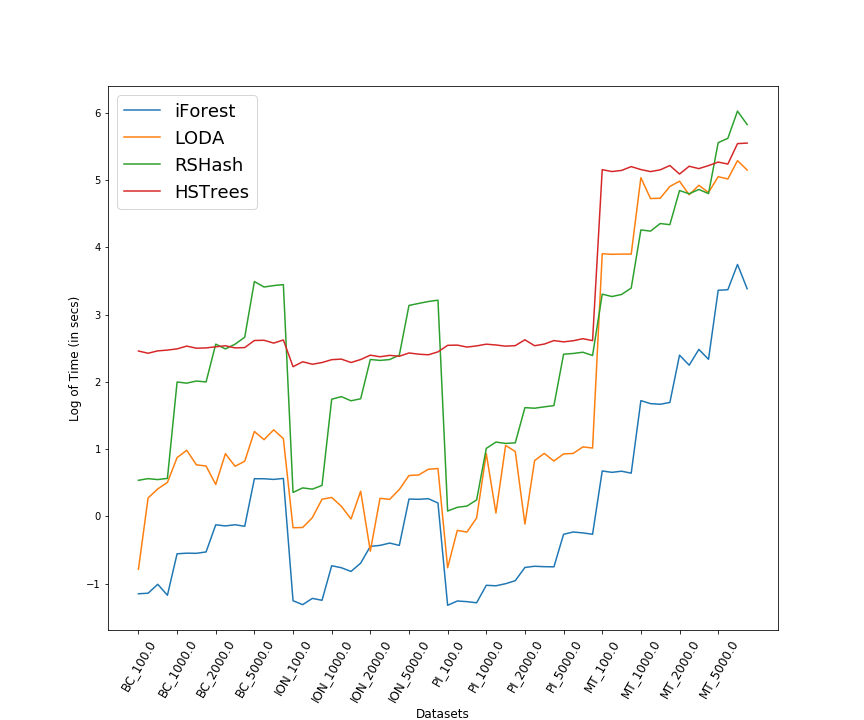
\includegraphics[width=\linewidth]{fig/baseline/TimeAnalysis_LowDim.png}
        \caption{Low/Mid - dimensional dataset analysis}
    \end{subfigure}
    \hfill
    \begin{subfigure}[t]{0.48\textwidth}
        \centering
        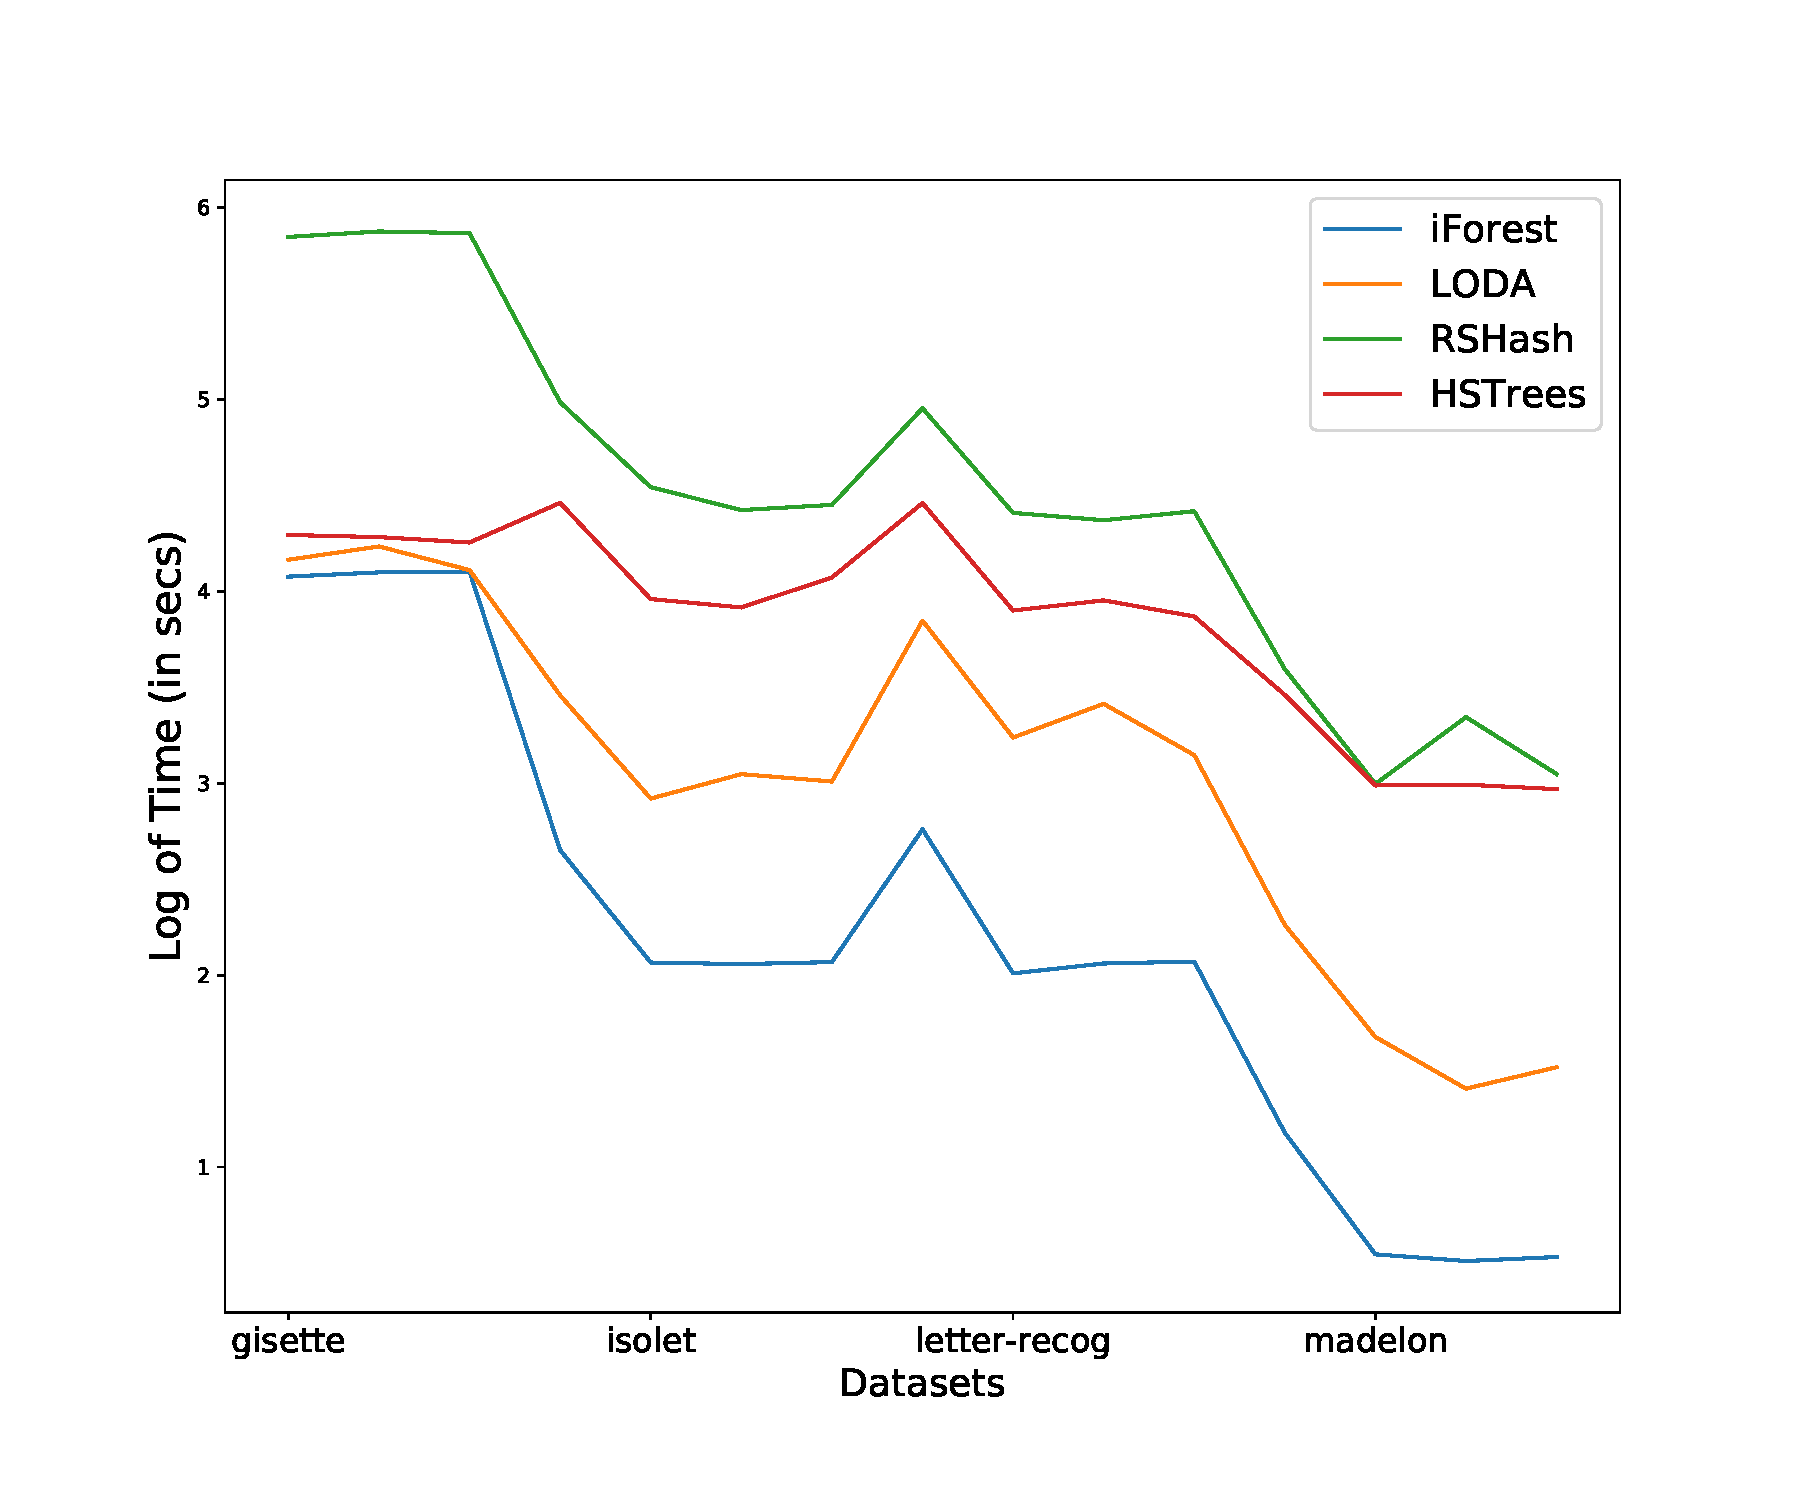
\includegraphics[width=\linewidth]{fig/baseline/TimeAnalysis_HighDim.pdf}
        \caption{High dimensional dataset analysis}
    \end{subfigure}
		\hfill
    \caption{RunTimes of algorithms over datasets with different noise levels. X-axis is over different datasets with different noise levels. Y-axis is log of runtime (in seconds).}
\end{figure*}

\subsection{Streaming Baseline Setup}

\textbf{Datasets}:

We use the same datasets as in HighDimension case in static setting. We create $10$ shuffled versions for each dataset. The datasets could either be shuffled randomly or it could be clustered in time. For the clustered shuffled, the input also includes a clustering percentage, that is how much percentage of anomalies should be clustered in time. We currently do not experiment with clustered in time datasets.

\textbf{Algorithms}
\begin{itemize}
\item{RS-Hash}: We use decay constant to be $0.015$, and use first $256$ samples to setup the $100$ components, and then compute AUC/AP over time.
\item{HS-Trees}:
\item{LODA}:
\end{itemize}

\textbf{Results}

\begin{figure*}[ht!]
    \centering
    \begin{subfigure}[t]{0.48\textwidth}
        \centering
        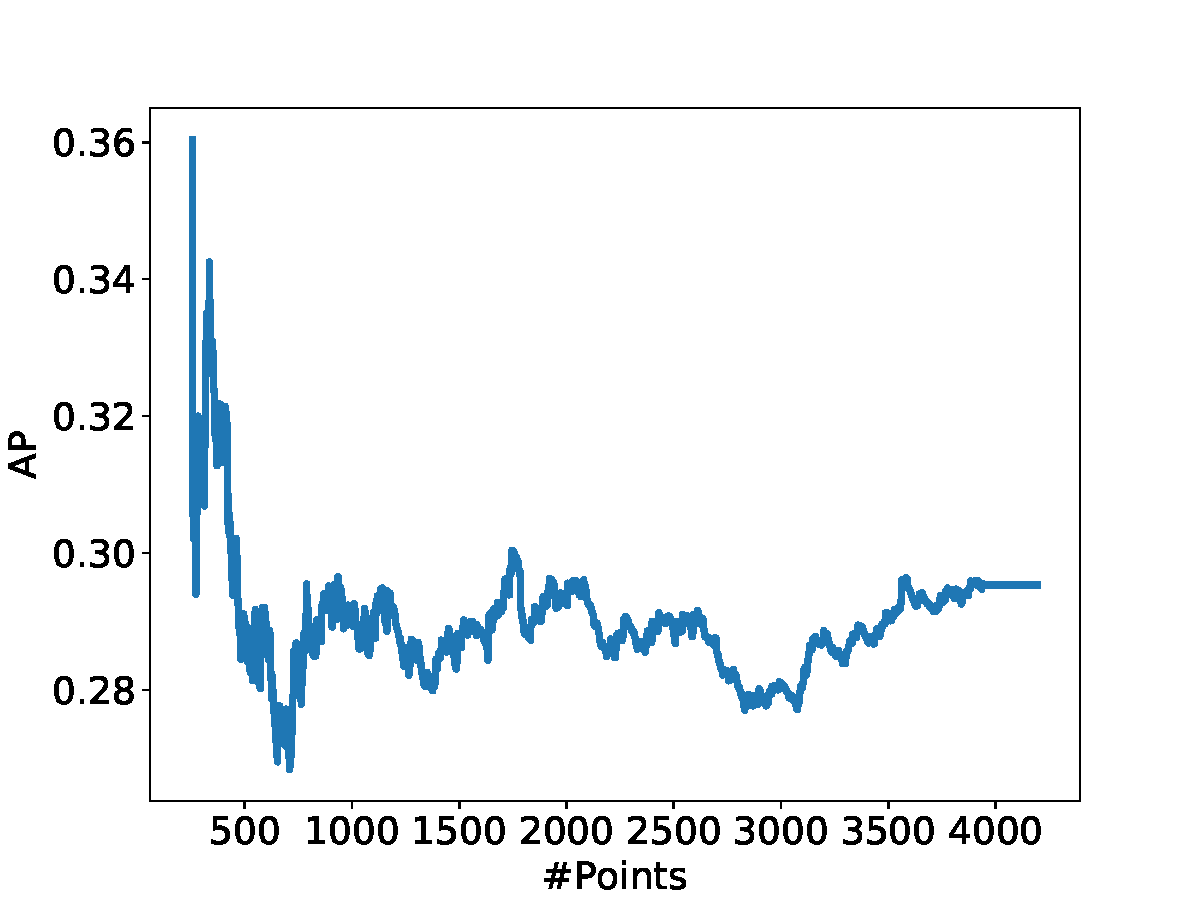
\includegraphics[width=\linewidth]{fig/streaming_baseline/letter-recognition.pdf}
        \caption{Low/Mid - dimensional dataset analysis}
    \end{subfigure}
    \hfill
    \begin{subfigure}[t]{0.48\textwidth}
        \centering
        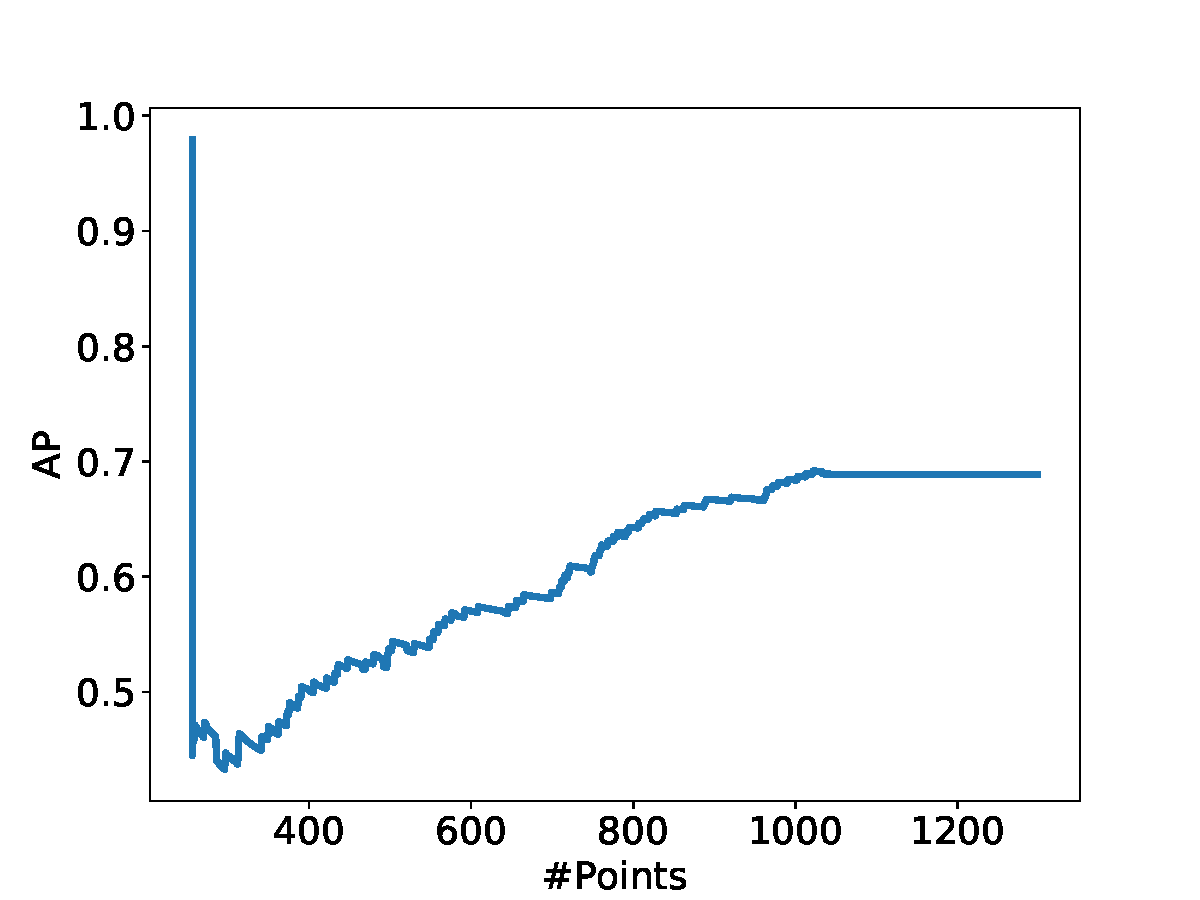
\includegraphics[width=\linewidth]{fig/streaming_baseline/madelon.pdf}
        \caption{High dimensional dataset analysis}
    \end{subfigure}
		\hfill
    \caption{AP for two of the baseline datasets over time, using RS-Hash Streaming Algorithm.}
\end{figure*}

% Using the median instead of the mean in eq. (6) improves performance slightly.
%
% \begin{table}[h!]
% 	\centering
% 	\begin{tabular}{lll}
% 		\toprule
% 		\textbf{Chain Parameters} & \textbf{Mean AP} & \textbf{Standard Deviation}\\
% 		\midrule
% 		$K=50, C=10$ & 0.830 & 0.096\\
% 		$K=50, C=50$ & 0.930 & 0.003\\
% 		$K=25, C=10$ & 0.804 & 0.076\\
% 		$K=25, C=50$ & 0.903 & 0.010\\
% 		\bottomrule
% 	\end{tabular}
% 	\caption{Chain AP stability across 5 runs, median instead of mean in eq. (6), $D=10$.}
% \end{table}

\pagebreak
